\subsection{Custom Components}\label{sub_sub_section:tgt_custom_components}

\subsubsection{Component Selection}\label{sub_sub_section:tgt_component_selection}


\paragraph{\gls{IMU}}
While the BMI323 is cheaper it has higher noise characteristics than the the ICM-42688-P, therefore the latter was selected for use on all boards due to its low price point and high performance. The use of the same \gls{IMU} over all modules should be maintained if possible so that the control characteristics are unchanged across devices and lower costs due to higher order quantities.
\paragraph{\gls{MCU}}
For the flight controller the STM32H743VGT6 is the best option given its \gls{RAM}, price point and support of dual \gls{CAN} buses. However, for the less computationally intense operations required for the \gls{GNSS} module the smaller footprint (due to the lower number of pins) and lower priced MSPM0G3506SRHBR is a better option.
\paragraph{\gls{GNSS} Module}
Exact positions for where the images were taken to cm precision is required as discussed in Section \ref{GPR_design}, this is possible using a \gls{RTK} setup with a base station sending out correction vectors over LoRa getting within centimetre accuracy\cite{RTK_LORA}. Furthermore, in the case of the loss of all \gls{GNSS} signal built in dead reckoning, allowing \gls{RTS}, is also a desirable feature. Therefore, the LG69T-AP is selected. However, when not executing imaging tasks, this precision is not needed and the modules are more expensive than the \gls{GNSS} modules without these features. Therefore, for the redundant device the MAX-F10S-00B was selected, and is shown in \ref{fig:custom_hardware_overview}, due to the significantly better documentation available and similar price points when compared to the LC29HAAMD.

\subsubsection{Power Supply}\label{sub_sub_section:tgt_power_supply}
\begin{table}[htbp]
  \centering
  \begin{tabular}{lrrr}
    \toprule
    \textbf{Component} & \textbf{Flight Controller} & \textbf{Redundant GNSS} & \textbf{Value}\\
    \textbf{} & \textbf{Quantity} & \textbf{Quantity} & \textbf{(mA)}\\ 
    \midrule
    ICM-42688-P\tablefootnote{\url{https://invensense.tdk.com/products/motion-tracking/6-axis/icm-42688-p/}} & 2  & 1 & 0.88\\
    STM32H743VGT6\tablefootnote{\url{https://www.st.com/en/microcontrollers-microprocessors/stm32h743vg.html}} & 1 & 0 & 165\\
    MSPM0G3506SRHBR\tablefootnote{\url{https://www.ti.com/product/MSPM0G3506/part-details/MSPM0G3506SRHBR}} & 0 & 1 & 8\\
    MAX-F10S-00B\tablefootnote{\url{https://www.u-blox.com/en/product/max-f10s-module}} & 0 & 1 & 200\\
    LEDs & 3 & 0 & 20 \\
    Misc & 1 & 1 & 20 \\ 
    \midrule
    \textbf{Total} & \textbf{246.76 mA} & \textbf{228.88 mA} & \textbf{}\\
    \bottomrule
  \end{tabular}
  \caption{Current Draws}
  \label{tab:current-draws}
\end{table}
\paragraph{Main Power Supply}
In both the GNSS module and the flight controller module the same power setup was used, created in Webench Power Designer\footnote{\url{https://webench.ti.com/power-designer/switching-regulator}}. The key decision metrics were efficiency and cost.  Efficiency is of high importance due to the thermal management on the board. The design selected has over 90\% efficiency \ref{fig:power_graphs} throughout the expected operating current window. As shown in the schematic \ref{fig:power_supply_schematic} there is a fuse to protect from short circuits and a \gls{TVS} diode to protect against \gls{ESD} that someone connecting the power might cause. There are also capacitors of 22uF and 4.7uF to provide current during spikes and smooth the power supply current.
\begin{figure}[htbp]
  \centering
  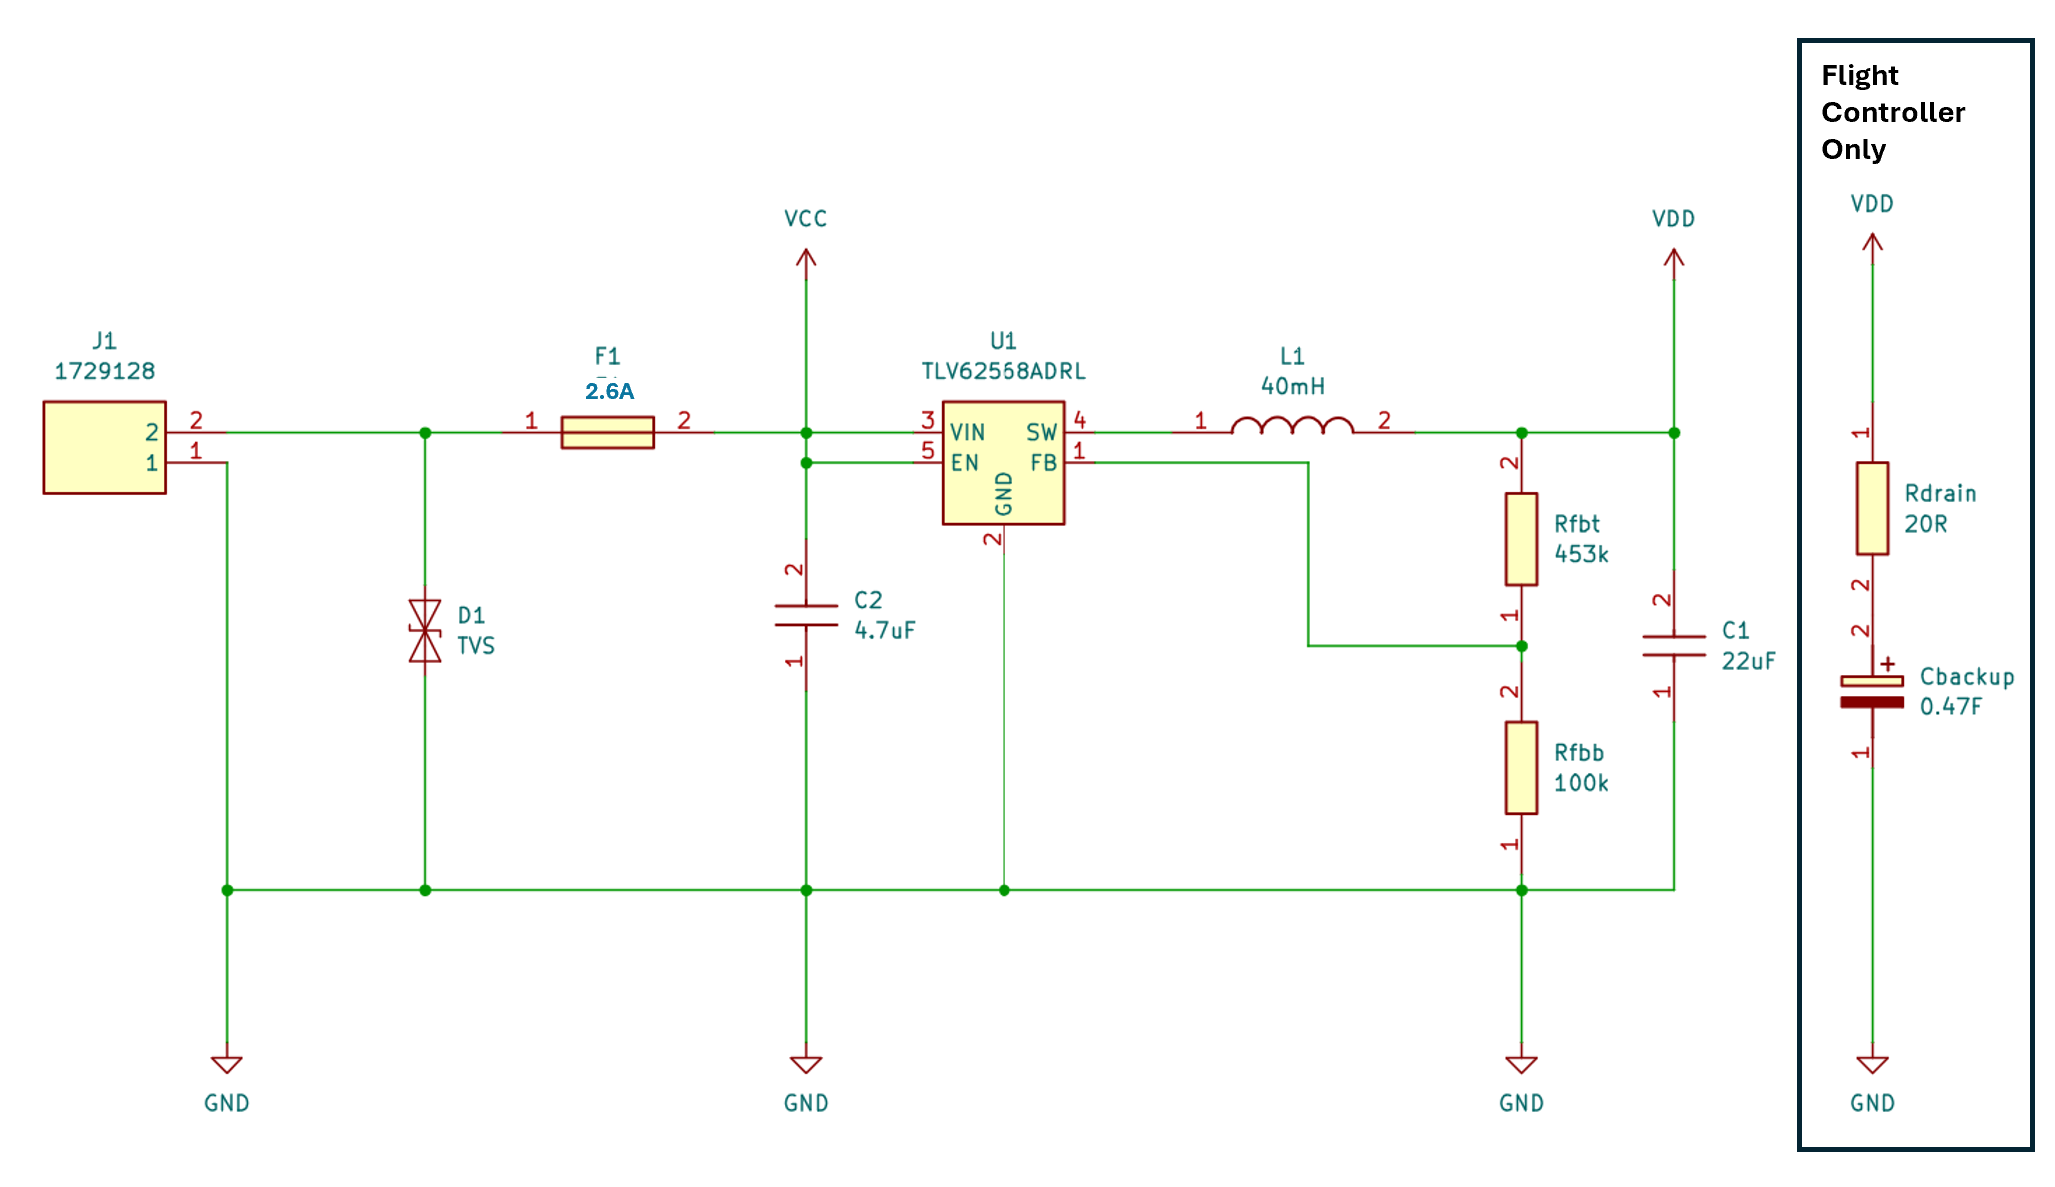
\includegraphics[width=\textwidth]{figs/Thomas/Custom Hardware/Power Supply.png}
  \caption{Power Supply Schematic}
  \label{fig:power_supply_schematic}
\end{figure}



\begin{figure}[htbp]
  \centering
  \begin{subfigure}[b]{0.48\textwidth}
    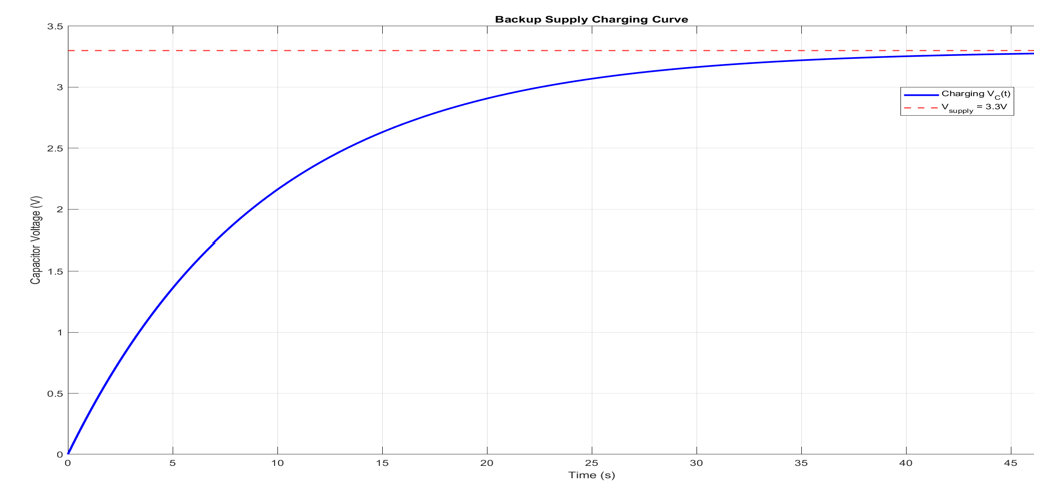
\includegraphics[width=\textwidth]{figs/Thomas/Custom Hardware/charging_curve.png}
    \caption{Backup Power Supply Charging Curve}
    \label{fig:charging_curve}
  \end{subfigure}
  \hfill
  \begin{subfigure}[b]{0.48\textwidth}
    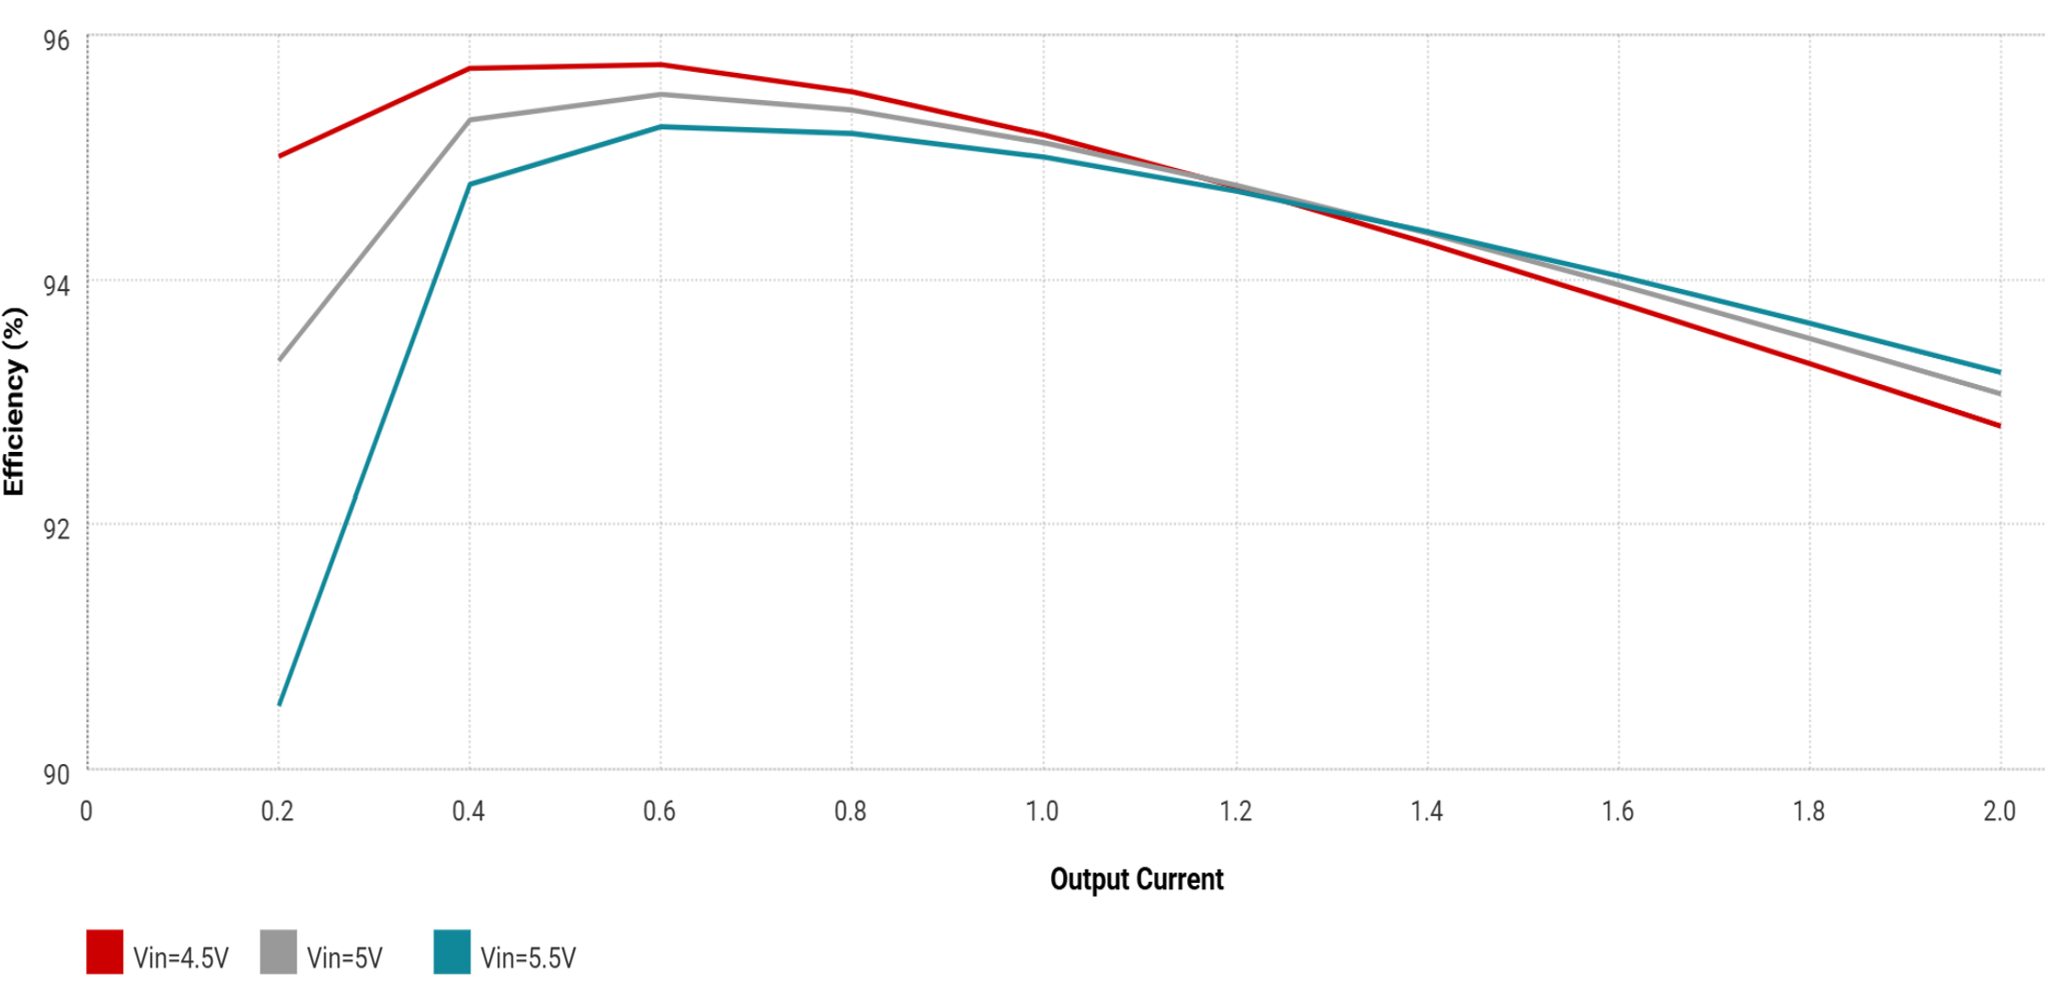
\includegraphics[width=\textwidth]{figs/Thomas/Custom Hardware/Power Module Effciency.png}
    \caption{Power Module Efficiency}
    \label{fig:power_efficiency}
  \end{subfigure}
  \caption{Custom Power Supply}
  \label{fig:power_graphs}
\end{figure}

\paragraph{Backup Power Supply}
The telemetry recordings of the flight controller are vital for crash analysis. However, in cases of sudden electrical failure the data recording will stop before writing the final state vectors and error codes. For example, if before a short circuit the current draw from an \gls{ESC} starts spiking that message needs to be recorded even if a fuse immediately burns shutting down the power supply. Therefore, a supercapacitor in series with a drain resistor is used \ref{fig:power_supply_schematic}. The capacitor selected is rated up to 5.4V at 0.47F\footnote{\url{https://uk.rs-online.com/web/p/supercapacitors/2506967}}. 
\begin{equation}
t = \frac{C \cdot (V_0 - V_{\text{cutoff}})}{I}
\label{eq:discharge_time}
\end{equation}
\begin{equation}
t_{\text{worst-case}} = \frac{0.47 \cdot (3.3 - 2.8)}{1} = 0.235\ \text{seconds}
\label{eq:worst_case_time}
\end{equation}
\begin{equation}
\tau = R \cdot C = 20 \cdot 0.47 = 9.4\ \text{seconds}
\label{eq:charging_time_constant}
\end{equation}
The time before dropout, with the worst case conditions is over 0.2 seconds \ref{eq:worst_case_time}, this will provide sufficient time to record any last messages. Furthermore, the time constant is 9.4s \ref{eq:charging_time_constant} meaning that there are current spikes when turning the device on but it is still charged over 3V within 30 seconds \ref{fig:charging_curve}.

\subsubsection{Comparison to Commercial Options}\label{sub_sub_section:tgt_commercial_options}
\begin{table}[htbp]
  \centering
  \begin{tabular}{|l|r|r|}
    \hline
    \textbf{Category}         & \textbf{Redundant GNSS Cost} & \textbf{Flight Controller Cost}\\ 
    \hline
    Passive Components        & £140.40  & £385.00\\
    Active Components         & £1699.10 & £1865.10\\
    Headers/Connectors        & £179.50  & £278.40\\
    PCB \& Assembly           & £262.14  & £334.04\\
    \hline
    \textbf{Total}            & £2281.14 & £2862.54\\
    \hline
  \end{tabular}
  \caption{Cost of custom component (100 units)}
  \label{tab:aggregated-cost}
\end{table}
The CUAV X7+\footnote{\url{https://store.cuav.net/shop/x7/}} GPS compatible option costs £339.75 and provides the same core functionality as the custom flight controller including dual \gls{CAN} ports. This can be combined with the flight controller compatible with the CUAV C-RTK 9Ps Positioning Module\footnote{\url{https://store.cuav.net/shop/c-rtk-9ps/}} that costs £332.91 for a drone-base station pair and provides \gls{RTK} \gls{GNSS}. This is a significant increase in cost however, it would not require development and may be a superior option in the testing phase. However, for deployment the custom components should be used given the cost implications and that the custom \gls{GNSS} module is fully control capable and the commercial option is not. 
